\listfiles
\documentclass[manuscript, review, screen]{acmart}
%\setcitestyle{super,sort&compress}
\citestyle{acmauthoryear}
\usepackage{graphicx}
\usepackage{amsmath, amsthm, amssymb}
\usepackage{amsfonts}
\usepackage{tabularx}
\usepackage{multirow}
\usepackage{booktabs}
\usepackage[printonlyused]{acronym}
\usepackage{paralist}
\usepackage{enumitem}
\usepackage{subcaption} 
\usepackage[ruled]{algorithm2e}
%\usepackage{algorithmic}

\setlist{nolistsep}

\newacro{PGCE}{Postgraduate Certificate of Education}
\newacro{UTToF}{User Tracking Time-of-Flight}

\newcommand{\tickYes}{\checkmark}
\newcommand{\crossNo}{$\times$}

% Metadata Information
% \acmJournal{TOCHI}
% \acmVolume{9}
% \acmNumber{4}
% \acmArticle{39}
% \acmYear{2018}
% \acmMonth{3}

% Copyright
%\setcopyright{acmcopyright}
\setcopyright{acmlicensed}
%\setcopyright{rightsretained}
%\setcopyright{usgov}
%\setcopyright{usgovmixed}
%\setcopyright{cagov}
%\setcopyright{cagovmixed}

% DOI
\acmDOI{}

% Document starts
\begin{document}
% Title portion
\title{Controlling Classroom Technology with Upper-Body Gestures
  {\emph{and}} Improving Upper-Body Gesture Controls for Teacher Use}

\author{James McNaughton}
%\orcid{}
\affiliation{%
  \institution{Durham University}
  \streetaddress{South Road}
  \city{Durham}
  \postcode{DH1 3LE}
  \country{UK}}
\email{j.a.mcnaughton@durham.ac.uk}
\author{Tom Crick}
\orcid{0000-0001-5196-9389}
\affiliation{%
  \institution{Cardiff Metropolitan University}
  \streetaddress{Western Avenue}
  \city{Cardiff}
  \postcode{CF5 2YB}
  \country{UK}}
\email{tcrick@cardiffmet.ac.uk}


\renewcommand\shortauthors{McNaughton, J. and Crick, T.}

\begin{abstract}
{\emph{Abstract 1:}} There is a growing need to give teachers the ability to remotely control computer interfaces in the classroom.
Existing techniques such as control through fixed interfaces, mobile devices or voice commands have a number of short comings.
The use of upper-body gestures to allow teachers to control classroom interfaces as an alternative is considered.
For this alternative control technique a set of gestures which are intuitive to teachers must be identified.
Focus groups were used to discover which gestures are intuitively performed for specific actions relating to controlling classroom interfaces.
This paper details the gestures observed and details their implementation into a classroom control system.
The results of a controlled study using the implemented gesture system indicate that upper-body gesture controls are quicker than alternative technologies.
However, the use of the Kinect in the gesture system's current implementation yields too high of an error rate for the results to be conclusive.

{\emph{Abstract 2:}} As computers become more prevalent in classrooms, the need for systems which allow teachers to effectively control them increases.
An open-air gesture based control system using the Microsoft Kinect was created which allowed teachers to control instances of the SynergyNet framework in classrooms.
Despite the open-air gesture controls being quicker and less intrusive on teacher-student interaction than alternative technologies, its use was made unsuitable for use in the classroom due to issues relating to its accuracy and intuitiveness.
A number of changes were implemented into the system in an attempt to resolve these issues.
These changes were; the use of multiple Kinects, creation of a point-to-select gesture, improvements to the control sequence and the creation of a more cohesive gesture set.
A controlled study took place to evaluate whether these changes made the use of open-air gestures a viable method of controlling classroom technology.
Despite a significant improvement to system's intuitiveness, the Kinect's accuracy was still the cause of a number of problems.
With the use of a more accurate sensing technology the system would be suitable for controlling classroom technologies.
%\\
%\\ 
% \textbf{RESEARCH HIGHLIGHTS:}\\
% \textbullet \ A framework for assessing upper-body gestures is presented. \ 
% \textbullet \ A list of gestures suited for use with the Kinect in a classroom is produced.  \ 
% \textbullet \ A system which uses the Kinect to allow teachers to control classroom technology is implemented.  \ 
% \textbullet \ Issues with the Kinect device and gesture set are shown to be problematic.
\end{abstract}


%
% The code below should be generated by the tool at
% http://dl.acm.org/ccs.cfm
% Please copy and paste the code instead of the example below.
%


%
% End generated code
%

\keywords{Kinect, gestures, education, classroom technology, control}

\maketitle

%-------------------------------------------------------------------------

\section{Introduction}
\label{sec:intro}

The uses of technology in the classroom are growing~\cite{Lloyd2011,Robertson2012,Schrum2008}.
With this growth, the need for teachers to be able to control the deployed technologies increases~\cite{Apple1990,Selwyn2010,Selwyn2011}.
Without the ability to influence or control classroom technology, teachers may be unable to manage learning interaction or intervene when students start to lose focus on their current task~\cite{Chen2005,Karabenick2011}.

% With technology becoming more prevalent in the classroom~\cite{Lloyd2011,Robertson2012,Schrum2008} the likelihood of there being a number of student-orientated interfaces present in the environment increases.
% Due to the student-orientated nature of these interfaces teachers may have difficulty in attaining students' attention or assisting them with tasks~\cite{Chen2005,Karabenick2011}.
% This is because control of these interfaces lies primarily in the hands of the student.
% There is therefore a need for teachers to have some degree of control over these interfaces~\cite{Apple1990,Selwyn2010,Selwyn2011}.

Many current systems that allow teachers to control technology in the classroom require the use of a teacher-centric interface~\cite{Dagdag2011,Kuhn2005,Vila,Zhou2010}.
Whether static, where the interface remains stationary during its use, or mobile, where the interface can be carried to new locations during its use, these interfaces require the teacher to momentarily take their attention away from the students.
This division of attention caused by the distraction of an interface could have a detrimental effect on the quality of a teacher's interaction with their students.
The disruption in communication between the students and the teacher this causes can be undesirable in many circumstances.
Therefore, a method of controlling technology in the classroom without breaking this interaction would be beneficial.
One such possible method is to make use of physical gestures, where a user performs an action which is identified by a monitoring system, to issue commands to technology in the classroom.

The use of gestures, rather than a more standard interface, could allow teachers to issue commands in a more effective manner.
Time is saved by not requiring the teacher to travel to their control interface.
Even when there is no travel time, such as when mobile interfaces are used, gestures have the potential to be executed quicker than alternative input and control methods~\cite{Dulberg1999,Moyle2001}.
Quicker execution of the commands should afford the teacher more time to observe and aid students.
In addition, physical gestures should be less intrusive on the interaction between students and the teacher. 
Many interfaces, specifically touch-screen mobile devices such as tablets, do not facilitate eyes-free interaction~\cite{Brewster2003}.
This means that teachers using a static or mobile interface which utilises a visual output are required to dedicate a portion of their attention to its use.
This division of attention can interrupt interaction between teachers and students.
The use of physical gestures should allow teachers to continue interacting with students while issuing commands to a classroom technology's control system.

Teachers in technology enhanced classroom also acquire additional administration responsibilities~\cite{Kuhn2005} such as managing the consequence of faults with the devices used.
A physical gesture interface may reduce the overheads of such additional responsibilities by allowing teachers to quickly execute administrative tasks from any location in the classroom.

The potential benefits of physical gestures make its implementation into a classroom software framework desirable.
For a system such as this, a series of gestures must be produced which can be used to execute the various control commands within the framework.

% This paper focuses on SynergyNet~\cite{HatchA.HigginsS&Mercier2009}, a multi-touch framework intended for use in the classroom.
% The framework is built to support applications designed to be used by students through multi-touch interfaces.
% The SynergyNet lab, built around the framework's use, consists of a number of multi-touch tabletop surfaces and is arranged to resemble a classroom.
% The SynergyNet framework allows interaction between the multi-touch interfaces which enables the sharing of materials and the ability to issue commands through a network.
% The ability for commands to be sent across a network offers the opportunity for control to be remotely exerted over the tabletop interfaces.
% The SynergyNet framework has been augmented to use upper-body gestures, a subset of open-air gestures, to allow teachers to control classroom interfaces.
% However, previous studies have identified issues that make its use in the classroom unsuitable~\cite{McNaughton2013a}.

% The gesture controls enable the orchestration of several common-place commands, such as sending or retrieving materials.
% It is through that issues relating to the SynergyNet framework's upper-body gesture support may be present in similar open-air gesture driven systems.
% Therefore, any improvements which resolve the issues observed in the SynergyNet framework could be employed in other gesture systems. 
% These improvements have the potential to benefit any systems with similar technologies, control sequences or gesture sets.

The remainder of this paper is as follows. 
Section~\ref{sec:related} discusses gesture detection technologies, specifically time-of-flight cameras.
Section~\ref{sec:classcontrol} considers how the time-of-flight cameras could be used to adapt a classroom-based technology to utilise physical gestures.
What constitutes an effective gesture is discussed in Section~\ref{sec:gestures}.
A focus group based study is outlined in Section~\ref{sec:focusgroup} which was carried out to identify intuitive gestures for classroom control commands.
The results of the study are outlined in Section~\ref{sec:focusgroupresults} and their implications are discussed in Section~\ref{sec:discussion}. 
Implementation of a user generated set of gestures from observations on the focus group is detailed in Section~\ref{sec:implementation}.
Section~\ref{sec:evaluation} discusses a study using the implemented physical gesture control system.
Section~\ref{sec:evaluationresults} presents the results of this study and Section~\ref{sec:evaluationdiscussion} elaborates on the implications of the results.
Future developments utilising findings from the study and our conclusions are presented in Section~\ref{sec:conclusions}.

% The remainder of this paper is as follows. 
% Section~\ref{sec:related} discusses the existing control systems used in SynergyNet for issuing commands and current developments in using the Kinect to track open-air gestures.
% SynergyNet's support for upper-body gestures is discussed in detail in Section~\ref{sec:gestures}.
% The issues observed in SynergyNet's current gesture control system are outlined in Section~\ref{sec:issues}.
% Potential solutions used in other works to resolve these issues are discussed Section~\ref{sec:improvements}.
% Section~\ref{sec:implementation} details how improvements were implemented into the SynergyNet framework to resolve these issues.
% A user study is then outlined in Section~\ref{sec:study} which was carried out to assess the improved gesture system alongside the existing control technologies.
% The results of the study are outlined in Section~\ref{sec:results} and their implications are discussed in Section~\ref{sec:discussion}.
% Future developments utilising findings from the study and our conclusions are presented in Section~\ref{sec:conclusion}.

%-------------------------------------------------------------------------

\section{Background} 
\label{sec:related}

To allow a system to identify physical gestures a method of tracking the movements of users is required.
Time-of-flight cameras~\cite{Lange2001} are capable of doing this through building a depth image of an environment and tracking movement by identifying areas where the depth values change.
The Canesta~\cite{Yang2007} and 3DV~\cite{Wilson2007a} devices are both examples of these cameras.
The devices emit beams of infra-red light which can then be seen through an infra-red camera.
Using knowledge of the infra-red light emitted, the devices can identify where the beams are interrupted by an object.
This positional information allows the devices to build a depth image of an environment.
Thus, devices can identify the distance between itself and any item within the range of its infra-red beams.
However, both the Canesta~\cite{Yang2007} and 3DV~\cite{Wilson2007a} devices provide a low quality depth image.
There are alternatives which provide much more detailed depth images, such as Oblong's Mezzanine~\cite{kramer2011}.
However, the cost of the alternatives can also be prohibitive.
Devices which occupy the middle-ground between quality depth images and cost are also available.
Such devices include the Microsoft Kinect, shown in Figure~\ref{fig:kinect} and the Primesense sensor~\cite{Wilson2010}.
These devices are accurate enough to track user movement and have previously been used as part of gesture monitoring systems~\cite{Goth2011}.

\begin{figure}[h]
   \centering
   \includegraphics[width=0.45\textwidth]{figures/kinect.png}
   \caption{The Microsoft Kinect.}
   \label{fig:kinect}
\end{figure}

The firmware of \ac{UTToF} cameras, like the Kinect and Primesense sensor, offer several features relating to the tracking of a user.
These devices can outline any persons in front of the device and differentiate between them using their distances from the camera.
The device can then identify and give positional information on specific parts of a person's body, such as their limbs and joints if a calibration technique is executed.
This is usually a pose assumed by a person which allows the device to view a specific human outline from which it can identify joints and limbs~\cite{Xia2011}.
Using the difference between frames from the depth camera, the device's firmware can track the movement of people in its field of view.

The information a \ac{UTToF} camera can give concerning the positions of a person and their limbs offers a wealth of possibilities regarding computer interaction.
Specifically, the ability to obtain the positional information of people may be of use for co-located interfaces where interaction may require knowledge of the position of the user.
The ability to track and differentiate between users comes in useful for interaction technologies which allow users to share interfaces.
Dietz and Leigh~\cite{Dietz2001} note how the ability to track a user can be important.
Their research also identifies how existing techniques for tracking user positions which entail encumbering the user with extra devices are undesirable.
\ac{UTToF} cameras offer the opportunity to track people without the need for users to wear additional devices.

\ac{UTToF} cameras allow users to move about an environment without being constrained to an interface.
This is beneficial for teachers in classroom environment for whom mobility is vital.
There are alternatives to physical gesture sensing technologies, like \ac{UTToF} cameras, which also afford this type of freedom from the interface.
Voice control is one such alternative where the teacher could issue commands to a technological framework in the classroom through a series of spoken instructions.
Using physical gestures alongside the voice commands could be beneficial as shown in the work of Bolt~\citeyearpar{Bolt1980}.
Allowing the user to gesture at where they want a specific command to influence reduces the need for additional spoken instructions.
However, the ambient noise in a typical classroom is likely to be too loud for voice recognition technologies~\cite{Cavalier1996,Goette1998,OHare1999}.
In addition to this caveat, the issuing of voice commands also will require teachers to interrupt their conversations with their students.

The use of physical gestures monitored via a \ac{UTToF} camera appears to be the most suitable approach to creating a system which allows teachers to control classroom technologies without the requirement for a distracting interface.

%-------------------------------------------------------------------------

% \section{Background} 
% \label{sec:related}

% %\begin{figure}[h]
% %   \centering
% %   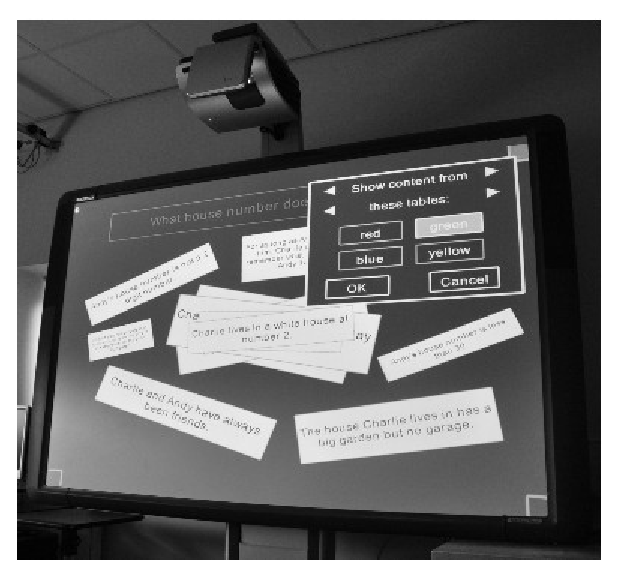
\includegraphics[width=0.45\textwidth]{fig1.eps}
% %   \caption{The multi-touch board used to control SynergyNet.}
% %   \label{fig:controlBoard}
% %\end{figure}

% SynergyNet supports numerous control technologies which teachers can use to control instances of the framework on student-centric multi-touch interfaces.
% The first of these supported technologies is a multi-touch interface.
% The teacher controls used for this technology are implemented as a typical SynergyNet application.
% This allows the teacher to use any multi-touch device capable of running the framework to control the environment's student-centric interfaces.
% This set of teacher controls has been made available to teachers in the SynergyNet lab through one of two multi-touch devices; a board and a podium.

% The multi-touch board used in the SynergyNet lab for issuing commands to the students' interfaces is shown in Figure~\ref{fig:controlBoard} running an instance of the teacher controls.
% Both the podium and board devices are static.
% Due to this the teacher is required to be positioned in close proximity to them in order to issue any control commands.
% This requirement of the devices can be detrimental on interaction between the teacher and students.
% This is because whenever the teacher wishes to issue a control command they will be required move away from the students to one of the devices.
% The time taken to travel to the device can prolong the break in interaction between the students and the teacher.

% %\begin{figure}[h]
% %   \centering
% %   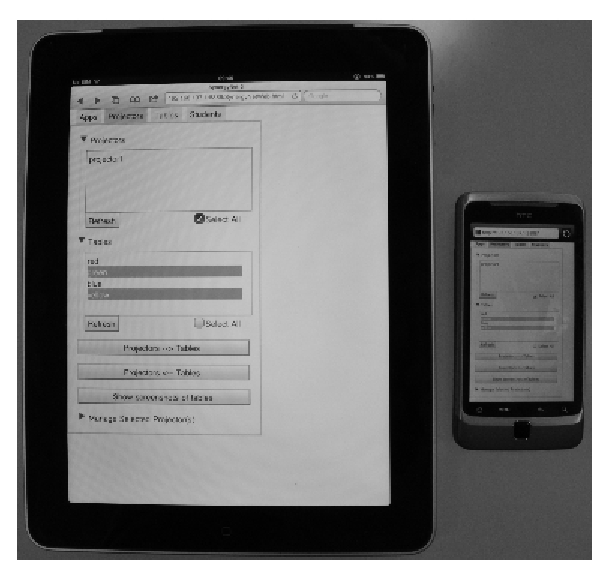
\includegraphics[width=0.45\textwidth]{fig2.eps}
% %   \caption{The web interface which controls SynergyNet accessed through a tablet device.}
% %   \label{fig:controlTablet}
% %\end{figure}

% To resolve the potential problem of breaking interaction with students to issue commands through static interfaces, controls which can be accessed through a range of mobile devices were implemented into SynergyNet.
% These controls, shown in Figure~\ref{fig:controlTablet}, are built to be accessed through any device capable of joining a wireless network and displaying web-based content.
% The controls can be accessed by teachers through devices such as smart-phones and tablets.
% Despite the mobile nature of these interfaces, they have been noted in previous studies~\cite{Hatch2011} to remove the teacher's attention from the students.
% Teachers were also noted to take a significant amount of time to issue commands through the mobile interface, prolonging the break in interaction with the students.
% The interaction between students and teachers is required to ensure that students stay on task and that teachers are able to monitor the student's performance \cite{Hall1968}.
% This break in interaction can be detrimental for both a student's ability to learn and the teacher's ability to maintain order in the classroom \cite{Shirley2010}.
% A system of control which allows teachers to quickly issue commands without interrupting their interaction with their students would be beneficial.

% Utilising open-air gestures could allow teachers to issue commands without the requirement to concentrate on an interface~\cite{Varona2009,Wachs2011}.
% The term \lq open-air gesture\rq\ is used to refer to gestures performed by users which do not require contact with an interface.

% %\begin{figure}[h]
% %   \centering
% %   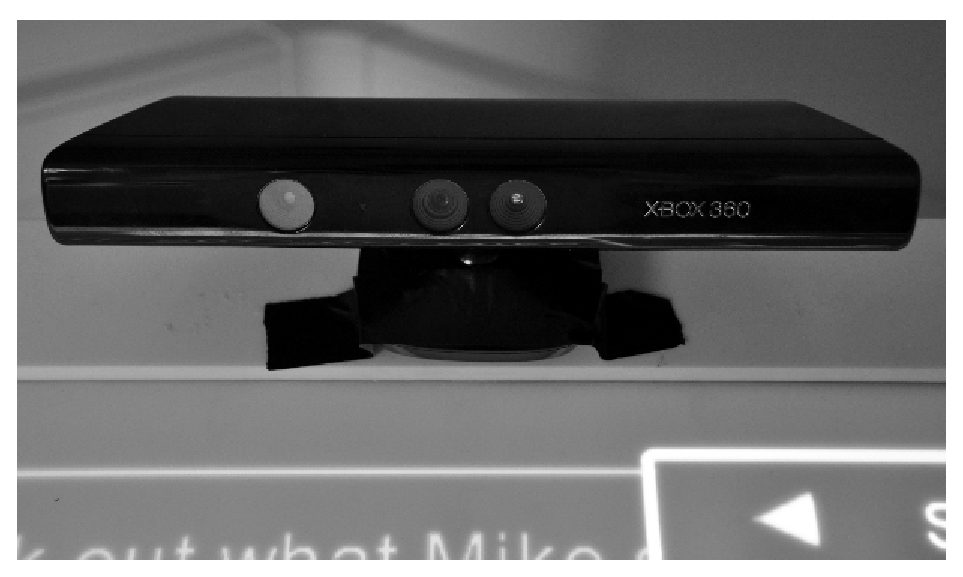
\includegraphics[width=0.45\textwidth]{fig3.eps}
% %   \caption{Microsoft's Kinect.}
% %   \label{fig:controlKinect}
% %\end{figure}

% The Microsoft Kinect, shown in Figure~\ref{fig:controlKinect}, can be used to support the detection of open-air gestures~\cite{Goth2011}.
% The Kinect is a low-cost device which is capable of capturing both RGB and depth information about an environment.
% The RGB data is captured through a typical visible light camera and the depth data through an infra-red camera. 
% The device projects an infra-red light pattern which the Kinect can see and identify.
% The Kinect can then use deformations of the pattern it views to identify surfaces and their distances from the device.
% This method of depth-sensing is known as a structured light pattern~\cite{Salvi2010}.
% Using both RGB and depth data the Kinect is capable of tracking persons about an environment.
% Once a person performs a calibration gesture, the Kinect is then capable of tracking that person's limbs and joints.

% Being able to track the location of a person's limbs and joints allows for a system to be built around the Kinect's output which can identify gestures performed by a user~\cite{Davison2012,Lai2012,Patsadu2012}.
% Once calibrated, a teacher could perform gestures which, when identified by the recognition system, would trigger the sending of commands to student-centric interfaces.
%-------------------------------------------------------------------------

\section{Classroom Control with Gestures}  
\label{sec:classcontrol}

The ability to track specific users and their limbs allows a \ac{UTToF} camera to be used for identifying body-orientated gestures.
This could allow teachers to control technology in the classroom without the need for an intermediate physical interface.
Teachers would not be encumbered with a device allowing them freedom to move about the classroom.
Since physical gestures would permit eyes-free interaction~\cite{Brewster2003} with a control system, teachers could interact with students without losing control of the technology.
Due to a \ac{UTToF} camera's ability to track people in an environment, once a teacher is identified their movement around the classroom can be followed.
As a result of this, teachers could potentially issue commands through gestures anywhere in the classroom.

\ac{UTToF} cameras have high availability and relatively low cost in comparison to alternative depth sensing devices such as those used in Oblong's Mezzanine~\cite{kramer2011}.
Despite these potential benefits of \ac{UTToF} camera, there are several limitations that must be considered.
One limitation is their accuracy.
\ac{UTToF} cameras are capable of tracking users and the position of their limbs.
However, for a \ac{UTToF} camera to track anything more precise, such as fingers, additional constraints on their abilities will need to be imposed \cite{Clark2011}.
These additional limitations potentially include a reduction in range, a reduced limit on the number of tracked users and the use of encumbering devices.
All these limitations are undesirable for the use of the device in the classroom.
Therefore, in the work discussed here, \ac{UTToF} camera will be assumed not be augmented to track anything more precise than user limbs.
This means that any gestures to be used by teachers for issuing control commands should consist of limb positioning and movement.

\begin{figure}[t]
   \centering
   \includegraphics[width=0.45\textwidth]{figures/gestures_venn_diagram.png}
   \caption{The hierarchy and intersection of physical gesture sets.}
   \label{fig:gestureVenn}
\end{figure}

Figure~\ref{fig:gestureVenn} represents the different sub-sets of physical gestures.
The inability of an un-augmented \ac{UTToF} camera to track anything more precise than user limbs discounts the adoption of gesture sets 4 and 5, i.e. gestures which use fingers, for use in the classroom.
Any gesture which lies outside the grouping of those which can be identified by a \ac{UTToF} camera must be discounted.
This results in gestures sets 1, 2 and 3 also being deemed unsuitable for classroom use.

There are several reasons for gestures involving the use of the lower body limbs and joints, such as the legs, to be discounted.
One such reason is their requirement for the visibility of the lower body.
In a classroom full of furniture and seated students, the teacher's lower body will potentially be obscured most of the time from the view of the \ac{UTToF} camera.
The requirement for a teacher to move to a position where their lower body is visible to the \ac{UTToF} camera counters the device's potential benefit of allowing for control of the system without the need to move away from students.

Another reason for discounting gestures using lower limbs and joints is that the movement of the teacher's legs may affect their balance which could result in accidents.
In addition to this, gestures utilising a teacher's legs may require the teacher to be standing when performing them.
This could interrupt interaction with students if the teacher is seated while in discussion with them.
Gestures which do not require teachers to stand would allow the teacher to issue commands while still being seated.
Due to these reasons, only gestures which utilise the positioning and movement of the upper-body should be considered when developing a classroom control system.
This means that gestures should only make use of upper-body joints and limbs which a \ac{UTToF} camera can track: the torso, wrists, hands, elbows, shoulders, neck and head.
Therefore, gesture sets 6 and 7 in Figure~\ref{fig:gestureVenn} are shown to be unsuitable for use in the classroom.

% \begin{table}[h]
% \processtable{Unique physical gesture sets.\label{table:gestures}}{
% \begin{tabular}{!{\vrule width 1.5pt}c|c|c|c|c!{\vrule width 1.5pt}}
% \noalign{\hrule height 1.5pt}
% \textbf{} 			&\textbf{Uses}	&\textbf{Uses}	&\textbf{} 	&\textbf{Visible to}	\\
% \textbf{Gesture} 	&\textbf{Upper-}	&\textbf{Lower-}	&\textbf{Uses} 	&\textbf{a \ac{UTToF}}	\\
% \textbf{Set} 		&\textbf{body} 	&\textbf{body} 	&\textbf{Fingers}	&\textbf{camera}			\\
% \cline{1-5}
% 1			&\tickYes 				&\crossNo			&\crossNo				&\crossNo			\\
% \cline{1-5}
% 2			& \crossNo				&\tickYes 			&\crossNo				&\crossNo			\\
% \cline{1-5}
% 3			&\tickYes  				&\tickYes 			&\crossNo				&\crossNo			\\
% \cline{1-5}
% 4			&\tickYes  				&\crossNo 			&\tickYes 				&\crossNo			\\
% \cline{1-5}
% 5			&\tickYes  				&\tickYes 			&\tickYes 				&\crossNo			\\
% \cline{1-5}
% 6			&\crossNo 				&\tickYes 			&\crossNo				&\tickYes 			\\
% \cline{1-5}
% 7			&\tickYes  				&\tickYes 			&\crossNo				&\tickYes 			\\
% \noalign{\hrule height 1.5pt}
% 8 			&\tickYes  				&\crossNo 			&\crossNo				&\tickYes 			\\
% \noalign{\hrule height 1.5pt}
% \end{tabular}}{}
% \end{table}


As Table~\ref{table:gestures} shows, only gesture set 8 is suitable for use by a teacher in a classroom environment.
All other gesture sets have been discounted due to their use of lower body limbs or inability to be identified by a \ac{UTToF} camera.
Gesture set 8 consists of gestures which can be observed by a \ac{UTToF} camera that use the upper-body but not the lower-body or fingers.

\subsection{Potential Issues}  
\label{sec:attention}

The use of physical gestures in the classroom requires that several potential issues are accommodated for in the design of any system which supports them.

\subsubsection{False Positives}  
\label{sec:attention}

A potential issue concerning \ac{UTToF} cameras are that, by default, they are active at all times.
This means that teachers will need to be mindful of their actions.
Expressive body language or movement around the classroom could be interpreted by a \ac{UTToF} camera as a gesture.
This may trigger unwanted responses from any system utilising the device.
Therefore, a method of dismissing a \ac{UTToF} camera's attention and recapturing it later would be beneficial 
One potential solution to these false positives is to have designated areas from which gestures should be made.
This would allow teachers to move outside these areas without the possibility of accidentally issuing a command.
However, this solution does restrict the locations where the commands can be issues from, diminishing the ability of teachers to issue commands from anywhere.

A gesture based method of toggling a \ac{UTToF} camera's attention is another potential solution to the issue of a teacher unintentionally issuing commands through their movement in the classroom.
The \ac{UTToF} camera will not be able to issue any commands to a classroom technology unless its attention has been obtained by the teacher.
This results in the \ac{UTToF} camera used having two states: attentive and inattentive.
A gesture could be setup to be identified by the \ac{UTToF} camera in both states.
This gesture can be used to toggle state.
This diminishes the range of possible false gestures to one.
The solution reduces the chances of a teacher unintentionally issuing commands and allows for control over the \ac{UTToF} camera anywhere in the environment.
If this solution is adopted it is important to identify the gesture for gaining and dismissing the \ac{UTToF} camera's attention.

A potential drawback with the attention-toggling approach of managing these false positives is that if a teacher intentionally performs a gesture without getting the device's attention they will be ignored.
A false negative is preferable to a false positive because an unintended gesture may have irrecoverable consequences.
A false positive will have no consequence other than requiring the teacher to repeat their gesture again with the attention of the \ac{UTToF} camera.
Despite not being as problematic as the potential consequences of a false positive, the time-wasting result of a false negative is a potential issue.
A method of ensuring that a teacher knows whether they have the \ac{UTToF} camera's attention would be beneficial in stopping false negatives if the attention-toggling approach is taken.
Audible or visual feedback would aid the teacher in knowing whether their movement can or cannot be interpreted by the system as a gesture.

\subsubsection{Interface Selection}  
\label{sec:selection}

It is important to note that sometimes a teacher may not want to affect all interfaces when issuing a command.
This means that the teacher should be able to perform a gesture in such a way that the system is informed that the related action is intended to only affect specific interfaces.
A \ac{UTToF} camera's ability to track users can allow for the system to be informed of the location of a teacher in relation to the interfaces in the classroom.
Therefore, the teacher's proximity to interfaces could be used by a system to identify which devices a command should affect if informed of their locations.
However, the drawback to this approach is that if the teacher wishes to influence multiple interfaces they will be required to repeat the gesture in close proximity to each of the target interface.
This requires the teacher to move about the classroom and may interrupt their interactions with the students.
Therefore, an alternative method of identifying which gestures should be affected by a command is desirable.

%-------------------------------------------------------------------------

% \section{SynergyNet and Upper-body Gesture Controls}  
% \label{sec:gestures}

% %\begin{figure*}[t]
% %   \centering
% %   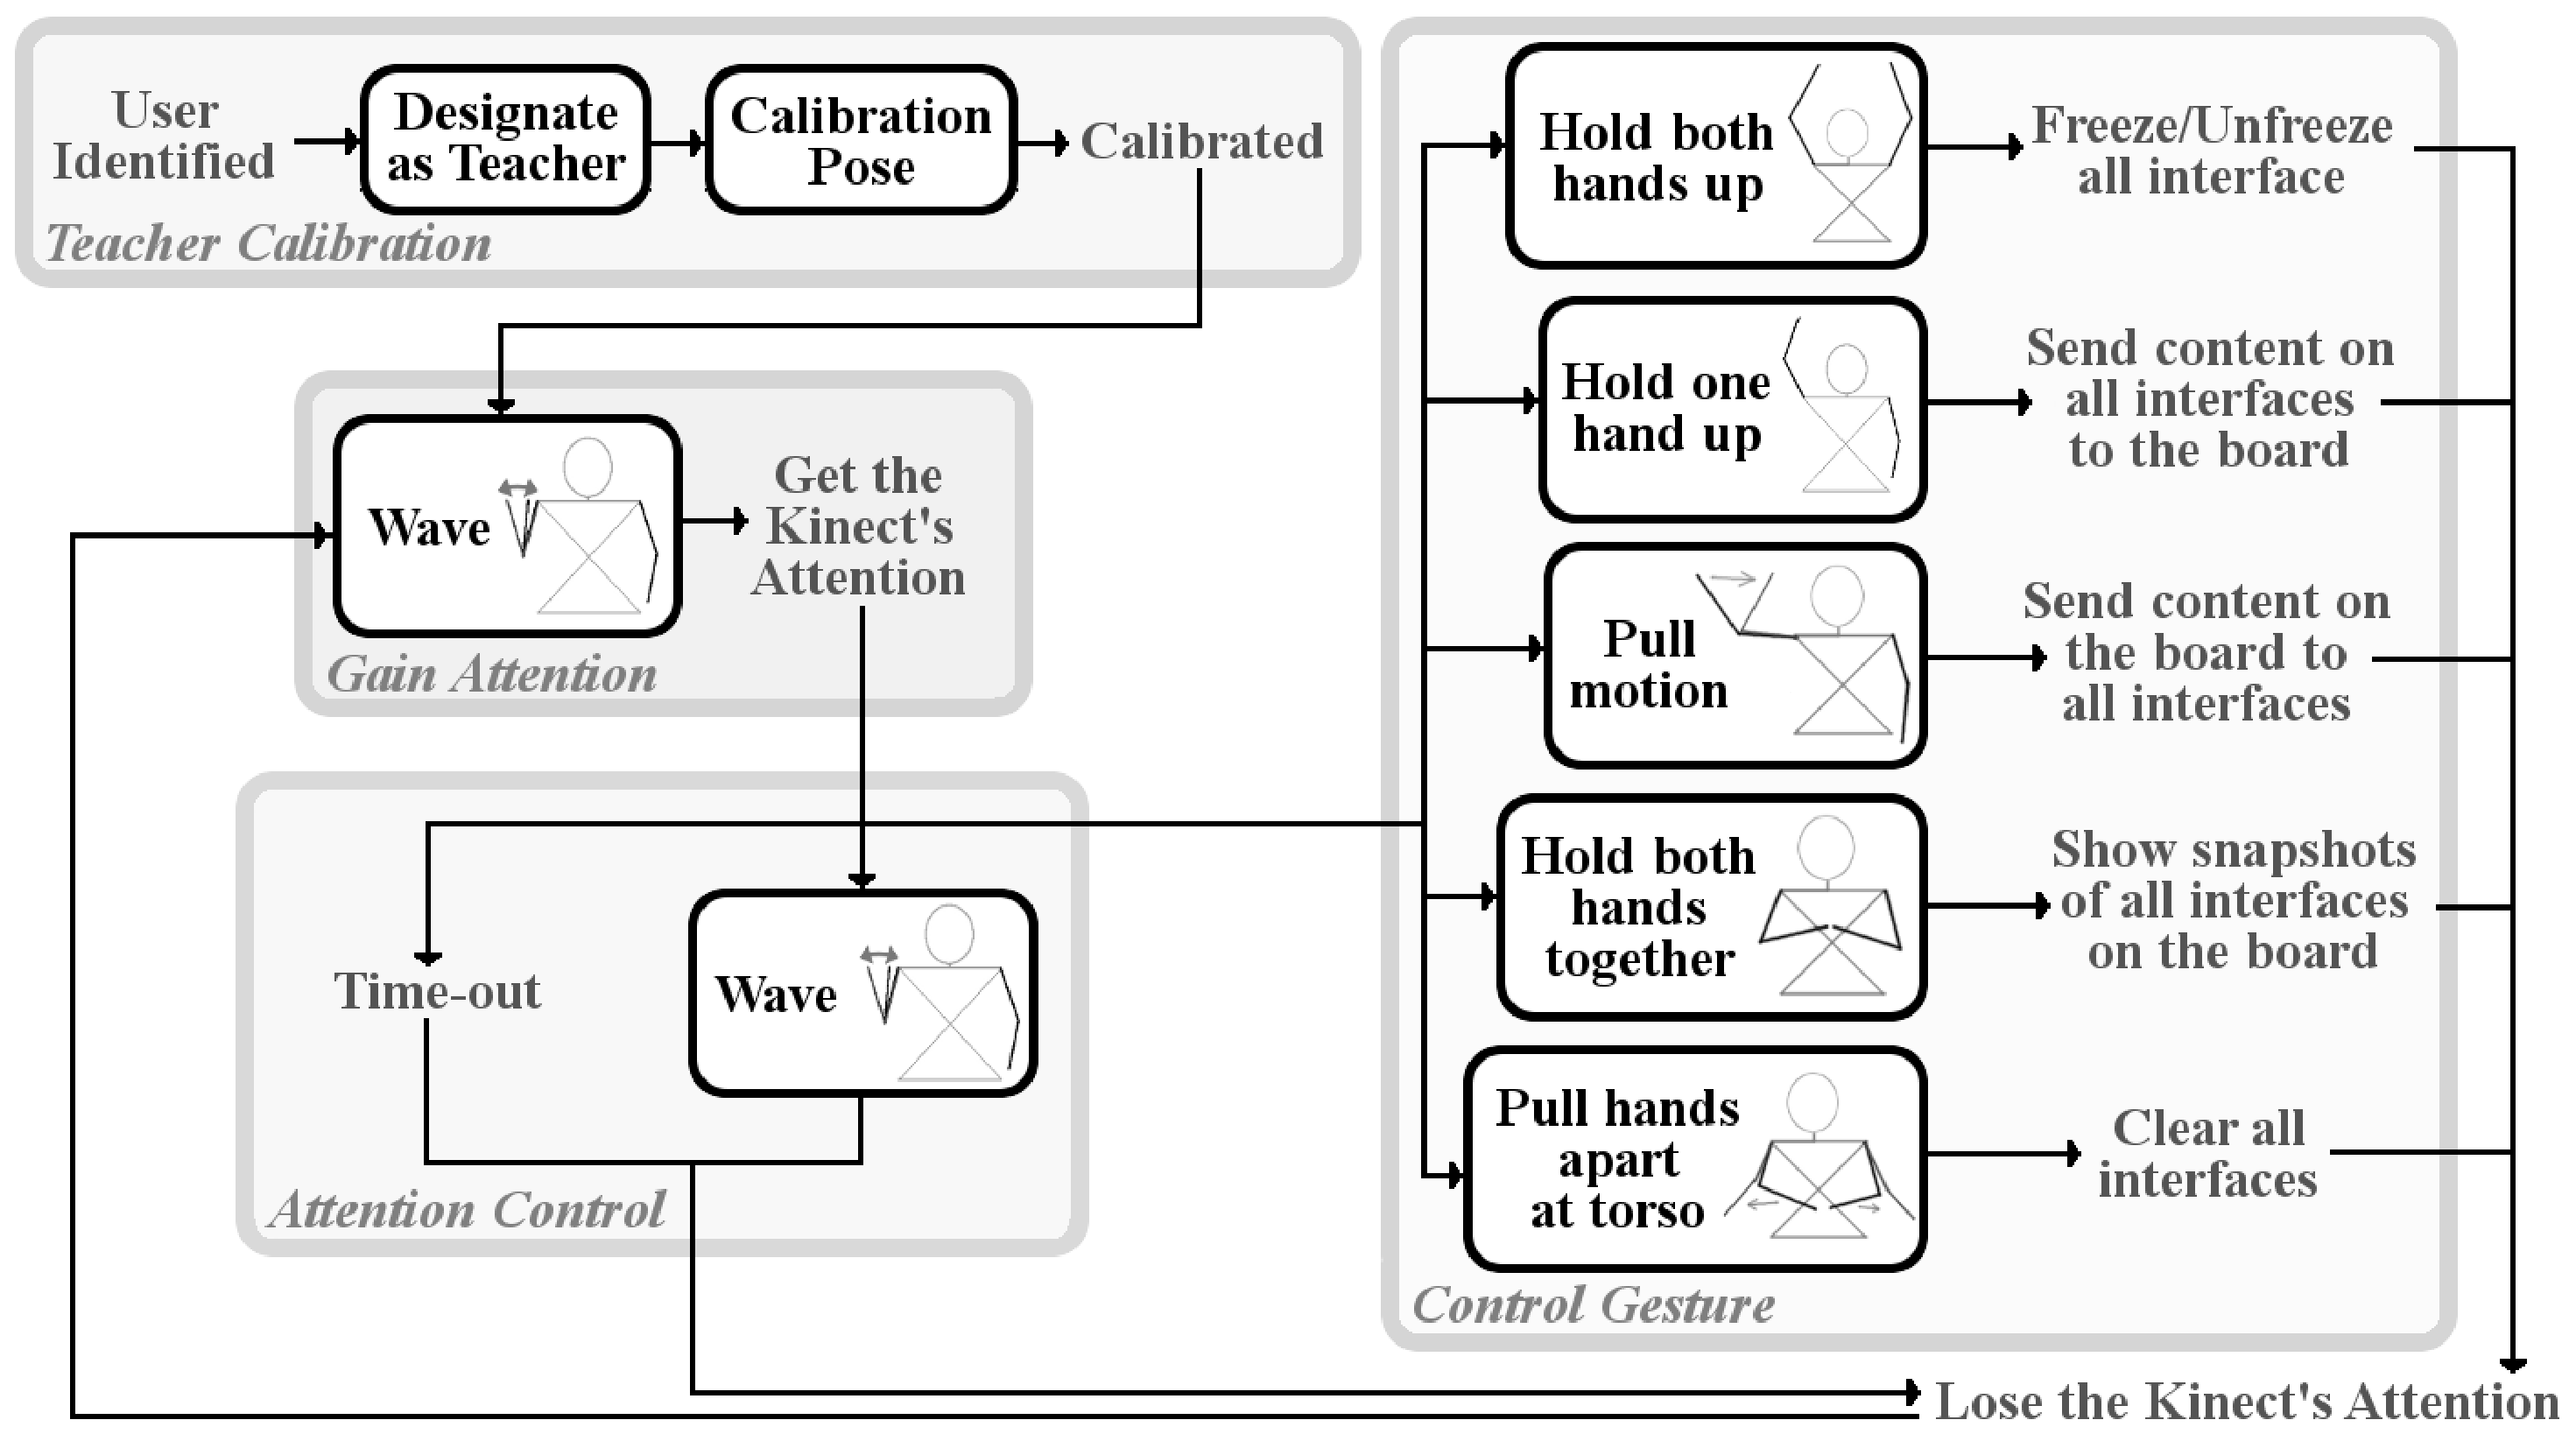
\includegraphics[width=1\textwidth]{fig4.eps}
% %   \caption{The existing control sequence implemented for the gesture controls in SynergyNet.}
% %   \label{fig:controlSequenceFlowDiagramOriginal}
% %\end{figure*}

% Using a set of gestures collated from a guessability study, a system for recognising gestures performed by a teacher was implemented into SynergyNet~\cite{McNaughton2013a}.
% This system can be used to issue specific commands to instances of the SynergyNet framework running on student-centric interfaces.

% The use of upper-body gestures to be used by SynergyNet was limited to those which could be performed with the joints and limbs of the upper-body.
% This includes the; torso, wrists, hands, elbows, shoulders, neck and head.
% The gestures do not include those which make use of the positioning or movement of fingers due to the loss of responsiveness required to support accurate finger tracking by the Kinect over large distances~\cite{Oikonomidis2011a,Oikonomidis2011b}.
% The issue of students and classroom furniture obscuring lower-body limbs and joints from the sensing device's view also led to the decision to exclusively use upper-body gestures.

% SynergyNet displays the current depth image collated by the Kinect as part of a GUI separate to any of the control systems.
% In this depth image identified persons are highlighted and labelled with the identification number allocated to them by the Kinect.
% Using these identifiers teachers can use the depth image to see discover the allocated number related to themselves.
% Through the GUI, teacher status can be granted to identified users with specific identification numbers.
% This allows the Kinect to be informed of which persons in the room are teachers.
% The Kinect will only look for gestures from persons who have been given a teacher status.

% Once a teacher is calibrated the Kinect can identify gestures through comparing the locations of limbs in relation to each other and their movement over time.
% Several of the gestures used by the SynergyNet framework are simple poses where a teacher will hold a specific limb or joint in position for a length of time.
% The remainder of the gestures used by the framework are defined by sequences of poses.

% Figure~\ref{fig:controlSequenceFlowDiagramOriginal} demonstrates the control sequence implemented into SynergyNet through which teachers can issue commands to instances of the framework.
% To avoid the possibility of teachers performing gestures when they don't intend to, a method of gaining and dismissing the attention of the Kinect through a waving gesture was implemented.
% After gaining the Kinect's attention, the teacher then has a choice.
% They can choose to dismiss the device's attention through waving if they wish to do nothing.
% This option is likely to be used when a teacher accidentally performs a wave gesture and acquires the Kinect's attention by mistake.
% Otherwise the teacher can then perform a command gesture.
% If a teacher does this, the corresponding command will be applied to all student-centric interfaces.

%-------------------------------------------------------------------------

\section{Gauging Gesture Suitability} 
\label{sec:gestures}

The requirements of the set of gestures to be used by teachers in the classroom are determined by both the shortcomings of the sensing technology, as discussed in Section~\ref{sec:classcontrol}, and the abilities of the intended users.
Specifically, the set of gestures for controlling classroom technologies are those which are able to be detected by a \ac{UTToF} camera and are suited to be performed by teachers.
With the potential set of suitable gestures already reduced to the upper-body by the requirements of using the sensing technology in a classroom environment, there is now the task of identifying which gestures to use and with which controls.
It is important that the selected gestures are intuitive~\cite{Cohen,Wachs2011}.
This will allow teachers to easily remember gestures and perform them with minimal forethought.
If the number of gestures to be used with the system is too large, the difficulty of committing them to and recalling them from memory may result in the teacher committing errors.
This may result in frustration with the systems use~\cite{Mendoza2005}.

Prior to use of a classroom technology control system which uses upper-body gestures teachers should receive training.
The training should at least ensure that the teacher is capable of recalling all the gestures used in the system and their associated commands.

It is important to note that to facilitate the use of the system; teachers should not be laden with too many gestures to remember.
The typical adult can remember seven items in a list, give or take two, in their short term memory~\cite{mil56}.
Relying on committing a greater number of commands to long term memory is undesirable since it counters the benefit that intuitive gestures offer of being quick to learn and use.
If there are too many gestures to recall from short term memory, teachers may have to rely on instructions sheets which would cause the same issues as the use as mobile interfaces where their attention is taken away from the students.

To compare possible sets of upper-body gestures for use with a system for controlling classroom technologies, a framework for assessing the gesture sets must be decided upon.
An exhaustive literature survey utilising a structured protocol~\cite{kitchenham04} revealed that no framework exists for the evaluation of the specific set of potential gestures relating to the upper-body.
Therefore, an evaluation framework used for a similar set of gestures was required to be identified and adapted to the upper-body set.

Grandhi et al.'s \citeyearpar{Grandhi2011} work relates to identifying physical open-air gestures.
As part of the work a study is carried out where a framework is used to assess the gestures performed by participants.
The gestures are categorised in the work by whether the action performed is pantomimic, where the user mimics a related real-world action, or uses a body part to represent a tool connected to a related real-world action.
The study was intended to find which of these categories held the more intuitive gestures.
To assess the intuitiveness of a gesture post session interviews were used.
The results indicated that the pantomimic gestures were more intuitively performed, though this conclusion is based on the opinions of the participants.
Gestures that were present in the study all appear to reside in the subset of hand-gestures.
However, the findings and approach to assessing the actions could be applied to a wider scope of gestures.

Nielsen et al.~\citeyearpar{Nielsen2004}'s work on procuring suitable sets of gestures for ergonomic interfaces entails the assessment of user gestures using a framework of characteristics.
This framework is derived from a combination of usability principles and heuristics derived from ergonomic theory.
The characteristics the framework uses for assessment are a gesture's; (i) ease to perform and recall, (ii) intuitiveness, (iii) logical metaphoric and iconic links towards functionality and (iv) ergonomic nature.

Waches et al.~\citeyearpar{Wachs2011} outline a series of requirements which systems using hand-gestures should adhere to.
The work goes into great detail on how each requirement is important, not only for the specific gesture set of hand actions but for physical gestures in general.
A number of these requirements echo the characteristics used in Nielsen et al.~\citeyearpar{Nielsen2004}'s work.
In addition to these are additional requirements which relate to the sensing technology used.
If these requirements are used in a framework it could be better suited to assessing a proposed gesture-based system as a whole, rather than just focusing on the gestures.
Therefore, it was decided that Waches et al.~\citeyearpar{Wachs2011} would be used to assess any proposed upper-body gesture systems.

The framework to assess potential upper-body gestures consists of a series of criteria which a suitable gesture set should completely fulfil.
Criteria relating to upper-body gesture sensing systems derived from Waches et al.'s~\citeyearpar{Wachs2011} requirements and how a typical \ac{UTToF} camera adheres to them are as follows:

\begin{itemize}
\item  \textit{\textbf{Cost:}} As detailed in Section~\ref{sec:classcontrol}, \ac{UTToF} cameras are relatively low cost.
\item \textit{\textbf{Responsiveness:}} The Kinect, a \ac{UTToF} camera, has a frame rate of 30Hz~\cite{Livingston2012} which is enough to be considered adequately responsive for tracking the movement of users.
\item \textit{\textbf{Adaptability:}} A typical \ac{UTToF} camera has the ability to be used by various supporting software frameworks which each allow for easy accessing of the device's collected data and functions~\cite{Goth2011}.
This allows \ac{UTToF} cameras to be easily adapted for changes in use.
The scalability of a single \ac{UTToF} camera  to track the joints and limbs of multiple persons is a demonstration of its ability to adapt to different numbers of users.
\item \textit{\textbf{Accuracy:}} The Kinect, a \ac{UTToF} camera, is noted to track user's limb and joints to 20mm when in range~\cite{Marquardt2011}. 
\item \textit{\textbf{Un-encumbering nature:}} When a user is required to wear a device for some purpose, the affiliated system is considered to be encumbering.
This can be undesirable as it detracts from a system's ubiquity and may impede use. 
Since a \ac{UTToF} camera can track users through a single static device which does not need to be worn it is considered to be un-encumbering.\\ 
\end{itemize}

One of Waches et al.'s~\citeyearpar{Wachs2011} requirements refers to the gesture set itself.
A criterion based on this requirement can be stated as follows:

\begin{itemize}
\item \textit{\textbf{Lexicon Size:}}  The size of the gesture set must not be too large.
This criterion can be adhered to by taking into account the limitations of short term memory.\\ 
\end{itemize}

The remainder of the requirements outlined by Waches et al.~\citeyearpar{Wachs2011} refer to requisites of the hand gestures themselves.
A summary of these criteria for upper-body gestures based on these requirements can be outlined as follows:

\begin{itemize}
\item \textit{\textbf{Intuitiveness:}} A gesture which a user performs naturally in relation to a specific command action is beneficial.
\item \textit{\textbf{Comfort:}} If a gesture is uncomfortable to perform a user is unlikely to perform it frequently, thus diminishing the benefit of the system.
\item \textit{\textbf{Low mental load:}} For a gesture to conform to this criterion a user should be able to perform it with little forethought.
\item \textit{\textbf{Interaction space:}} Gestures which require large amounts of space to be performed limit the locations it can be performed.
Therefore, to fulfil this requirement, gestures should minimise used space.
\item \textit{\textbf{Ubiquity:}} A gesture which does not appear to be in keeping with a user's typical actions in the current environment would not fulfil this criterion. \\ 
\end{itemize}

Using these criteria, any suggested gesture sets and their implementation can be assessed to be viable or not.
We use these \textit{upper-body gestures criteria} to assesses the gestures proposed for teacher use.

%-------------------------------------------------------------------------
% \section{Issues with Upper-body Gesture Controls}  
% \label{sec:issues}

% Previous studies involving the use of SynergyNet's upper-body gesture controls revealed several shortcomings~\cite{McNaughton2013a}.
% To assess the existing implementation a set of criteria for upper-body gestures was derived from the requirements for hand gestures outlined by Wachs et al.~\cite{Wachs2011}.
% These criteria assessed the system's cost, adaptability, accuracy, un-encumbering nature, responsiveness, lexicon size, intuitiveness, comfort, mental load, interaction space requirement and ubiquity.

% The previous study has revealed four criteria in which SynergyNet's upper-body gesture controls needs improvement; 
% \textit{accuracy}, \textit{interaction space}, \textit{intuitiveness} and \textit{mental load}.
% Using observations from the previous study it is possible to identify several issues which resulted in the system being incapable of meeting these three criteria.

% \subsection*{Issue 1: Losing Track of Users, Limbs and Joints}

% For SynergyNet, issues relating to accuracy and interaction space originated from the Kinect device.
% The device was noted to lose track of users which had the result of any persons carrying teacher status to lose their ability to issue commands.
% This would require the teacher to repeat designating their teacher status and performing the calibration pose.
% This was problematic due to its time consuming nature and was noted to occur when a teacher left the Kinect's field of vision.
% The Kinect's range is limited to three and a half metres~\cite{Maimone2011} and a sixty degree viewing angle~\cite{Stone2011}.
% This is too small to monitor an entire typical classroom environment.
% In addition to this the Kinect often lost track of teacher's limbs and joints.
% It was noted this occurred towards the limits of the Kinect's field of view.
% This was because the Kinect's accuracy decreases in proximity to the limits of its view~\cite{Mehrotra2011}.
% Gestures would either be interpreted incorrectly as other gestures or were totally ignored by the system due to this lack of accuracy.

% \subsection*{Issue 2: Gesture Confusion}

% SynergyNet's failure to meet the criterion for intuitiveness in the previous study was, in part, caused by repeated errors committed by the teacher performing the wrong gestures when intending to instigate specific commands~\cite{McNaughton2013a}.
% The teacher stated that they would often forget which gestures related to which command.
% This indicated that the gestures were not intuitive enough.
% In addition to this the teacher's confusion of gestures also attributed to the system's failure to meet the criterion for mental load.
% The teacher stated in an interview after the previous study that they forgot the gestures needed for specific commands on a number of occasions.

% \subsection*{Issue 3: Stringent Control Sequence Requirements}

% The numerous steps in the control sequence that the teacher is required to repeat on various occasions, such as calibration and establishing their identity, is a contributing factor to the system's failure to meet the criterion for mental load.
% SynergyNet's failure to meet the criterion for a low mental load was identified during previous use of the system where teachers would often pause during the command sequence~\cite{McNaughton2013a}.
% The control sequence required teachers to execute the command sequence without any pauses.
% This resulted in a number of errors where the Kinect's attention would time-out or the system would interpret the pose the teacher paused in as a command gesture.
% The teacher stated that they paused because they were concentrating on recalling the appropriate gesture for the command they intended to execute.
% This indicates that the mental load required by the current system implementation is too large.
% In addition to this the unexpected results of the system wrongfully interpreting gestures due to teacher's failing to meet the control sequence's stringent requirements are detrimental to its intuitiveness.

% \subsection*{Issue 4: Reduced Functionality}

% There may be circumstances where the teacher wishes their action to affect only a specific subset of the student's interfaces.
% The results of the guessability study performed to generate the initial upper-body gesture set and control sequence to be used by SynergyNet indicated a pattern in participant's preferences towards selection~\cite{McNaughton2013a}.
% It was noted that participants would prefer to point at specific interfaces if wishing a command to only affect them.
% A pointing gesture was proposed but not implemented due to the issue of a teacher's body potentially obscuring the interfaces being pointed when a single Kinect is used.
% Without an interface selection method, the Kinect controls offer less functionality than the alternative static and mobile interfaces.
% Because any command issued with the Kinect must influence all interfaces, teachers must put additional thought into its use.
% The lack of cohesion between the Kinect controls and alternatives may exacerbate the identified problems concerning intuitiveness and mental load.

%-------------------------------------------------------------------------

\section{Focus Group}  
\label{sec:focusgroup}

To discover gestures which conform to the criteria outlined in Section~\ref{sec:gestures} a user-centred design process was adopted.
As part of this process a user study in the form of a focus group was organised.
Through the focus group a user-generated set of viable upper-body gestures for use with a \ac{UTToF} camera was discovered.
The focus groups acted as a form of guessability study~\citep{Ruiz2011,Wobbrock2009} which would generate gestures which are natural to the user~\citep{Grandhi2011}.
User-generated gestures for surface computing are noted to be intuitive, comfortable, memorable and ubiquitous~\citep{Bjørneseth2012}.
These potential benefits of user-generated gestures adhere to the criteria relating to the definition of effective upper-body gestures.

The primary objective of this study was to find the quickest, most intuitive and least intrusive upper-body gestures which can be performed in the classroom to execute the most important control commands.

Three separate focus groups took place, each populated with students working towards a \ac{PGCE}.
\ac{PGCE} students were chosen because they were training towards careers in teaching.
This meant that they would share the same training experiences as most teachers.
All the participants had some experience of teacher in a classroom environment.
Therefore, \ac{PGCE} students may have similar considerations concerning gestures ubiquitous to the classroom.
In addition to this, gestures which are found to be intuitive to \ac{PGCE} students are likely to also be intuitive to teachers.

\begin{figure}[h]
   \centering
   \includegraphics[width=0.45\textwidth]{figures/synergynet_lab.png}
   \caption{The SynergyNet lab.}
   \label{fig:synergynetLab}
\end{figure}

Time constraints defined much of the study's design since the participating \ac{PGCE} were not able to stay on-site for more than a single morning.
It is due to the time constraints that an approach similar to that suggested by Nielsen et al.~\citeyearpar{Nielsen2004} could not be adopted.

The study took place in the SynergyNet lab, a laboratory designed to resemble a potential future technology enhanced classroom shown in Figure~\ref{fig:synergynetLab}.
The lab comprises of four tables with multi-touch interfaces embedded in their surfaces and an interactive whiteboard. 
The tabletop interfaces are intended to be viewed and used by individual groups of students whereas the board is intended to be visible to the entire class.
This is similar to more traditional classroom technology systems where students may have their own terminal or laptop in addition to a shared interface, either a interactive whiteboard or projection, for displaying materials to the class in general.
The lab is furnished with a range of recording apparatus which can capture audio and video from various locations around the classroom.
Participants were asked to position themselves in the room used in the study facing away from each other and towards the cameras recording the session.
The participants were positioned in this manner to reduce the influence that they would have on each other.
In each study a number of the participants were asked to stand and the rest were seated.
A list of commands that teachers using a classroom control system may need to issue was compiled.
The commands used were those for: 
\begin{itemize}
\item Freezing/Unfreezing student interfaces.
\item Sending contents of student interfaces to a shared interface.
\item Sending contents of a board interface to student interfaces.
\item Showing snapshots on the board interface of the student interfaces.
\item Clearing the student interfaces.\\
\end{itemize}

These commands were decided upon based on observations regarding the use of technology in the SynergyNet lab during previous studies~\citep{Hatch2011}.
The commands are ranked based on how frequently they were observed to be issued previously.

It was decided to adhere the lower bound of short term memory, discussed in Section~\ref{sec:gestures}, of five.
This relatively small gesture set conforms to the Wachs et al.'s~\citeyearpar{Wachs2011} requirement for a small lexicon size.

For each command participants were asked to perform the first gesture that they thought of which related to it.
Participants were asked not to put too much consideration into the gestures they performed.
This meant that the gestures performed were likely to be natural to the participant which is beneficial for finding gestures which conform to the criteria outlined in Section~\ref{sec:gestures}.
Spontaneous and frequently repeated gestures are assumed to be natural to the user and therefore are \textit{\textbf{intuitive}}~\citep{Grandhi2011}.
The intuitive nature of the gestures also implies that they are \textit{\textbf{comfortable}} for participants to perform.
Since participants were asked to put little thought into their motions, the gestures can also be said to have a \textit{\textbf{low mental load}}.
Since the participants were asked to perform the gestures while positioned next to others in the study there were limitations on how large their gestures could be.
This helped reduce the \textit{\textbf{interaction space}} that would be required when carrying out the gesture.
Participants were also asked to be mindful of the fact that these gestures would be performed in a classroom environment.
This was to ensure that the gestures suggested by participants would be in some way \textit{\textbf{ubiquitous}} to the classroom environment.

Participants in the study were asked to perform two gestures for each command.
The first gesture related to a command issued to all interfaces whereas the second related to a command intended for a specific selection of interfaces.
Participants were made aware that gestures should only use the upper-body but not fingers and that a gesture can either be a pose or movement.
Participants were also informed that when performing a gesture linked to specific interfaces, a teacher's proximity could be used to identify which interfaces would be affected.
Before commencing the study participants were informed that they should treat the camera recording the session as the device which would be tracking their movement.
This was to ensure participants would attempt to make their gestures visible to the camera.
This was beneficial for the recordings and for generating gestures which could be monitored by a \ac{UTToF} camera.

The original intention of the study was not to place constraints on the gestures performed by participants, then to repeat the study with the same participants with the constraints.
However, time restraints made the need for capturing usable gestures, i.e. those which conformed to the constraints, paramount.
Therefore, the unconstrained gesture capturing phase was not carried out in this study.

\subsection{Focus Group Data Analysis}
\label{subsec:analysis}  

Participants were recorded on video performing the gestures during the study.
Using the recordings, for each command all participants' movements could be studied and summarised as a sequence of poses and movements.
This allowed the participants' actions to be formalised as gestures.
These gestures could then be compared, allowing similar actions to be identified as being separate instances of the same gesture.
The gestures which were used most frequently for specific commands could be identified.
The most frequently occurring gesture for a command is likely to be the most intuitive since they will match the intended users' mental model of how the system should be used~\citep{Nielsen2004,Ruiz2011,Wobbrock2009}.

Each unique gesture performed during the study was identified.
Every gesture was first assessed using the limitations of a typical \ac{UTToF} camera.
Any gestures which did not conform to these limitations, such as those which used finger motions, were discounted.
Following this, the criteria outlined in Section~\ref{sec:gestures} were used to assess the gestures.
Any gesture which did not meet the criteria was also discounted.
The viable gestures observed in all of the focus groups were listed for each command alongside the number of participants which performed them.
The gesture with the highest number of occurrences for a specific command could then be established as the most likely to be intuitive to a teacher.

If more than one command had the same gesture with the highest number of occurrences, the gesture would be assigned to the command with the highest frequency of use observed in past studies~\citep{HatchA.HigginsS&Mercier2009}.
The less frequently used commands would then be assigned their gesture with the next highest number of occurrences.
This approach may confound the overall intuitiveness of the gesture set, however it enhances the intuitiveness of the more frequently used gestures.
This was gauged to be more important at the time of the study by the organisers.

It was decided that the attention toggling method of managing false positives, discussed in Section~\ref{sec:attention}, would be adopted due to its ability to reduce errors without placing constraints on where in an environment gestures can be performed.
Every effort was made to ensure participants' minds were kept clear of any assumptions about the system to aid the performance of intuitive gestures~\citep{Nielsen2004}.
As part of this effort it was decided that the participants should not be made aware of the toggle mechanic.
Therefore a separate collection for the toggle mechanic could not be used, instead the most frequently occurring gesture throughout the entire study was chosen.
Since this gesture potentially needs to be performed prior to any other command gesture, it will be the most frequently used in the system.
Therefore, it is important to ensure that it is intuitive and natural.

In addition to the ranking of gestures per action, the data analysis also aimed to identify how the participants differentiated gestures intended for all interfaces from those intended for specific interfaces.

%-------------------------------------------------------------------------
% \section{Potential Improvements}  
% \label{sec:improvements}

% The issues outlined in Section~\ref{sec:issues} were noted in the previous study to make the use of the system counter-productive~\cite{McNaughton2013a}.
% The benefits afforded by the system of non-intrusive and quick command execution were made irrelevant due to the high number of errors caused by the identified issues.
% Resolving these issues could allow the system to function as intended and would allow the potential benefits of the upper-body gesture controls to be evaluated and employed.

% \subsection{Resolving Issue 1: Improving the System's Tracking}
% \label{sec:improve_accuracy}

% To improve the accuracy and interaction space of the sensing technology used with the system, multiple Kinects could be employed.
% With more Kinect devices in the environment, more of the classroom would be monitored.
% A larger monitored area reduces the chance of the teacher losing their calibrated status by wandering out of the Kinects' view.
% This saves time by reducing how often the teacher needs to repeat the calibration process.

% Dubois et al.~\cite{Dubois2011} track the movement of mobile objects through an apartment using two Kinects.
% Using knowledge of the Kinects' positions relative to each other, their visual and depth information can be stitched together.
% Any processing applied to the information provided by the Kinect to track the movement of mobile objects can then be applied to the combined output.
% Stitching the information requires a large amount of processing power.
% However, once done it allows for the later process-intensive functions used to identify and track mobile objects to be applied just once, rather than having separate process-pipelines for each Kinect.

% Luber et al.~\cite{Luber2011} utilise multiple Kinects in their work to track persons across large environments.
% Through a form of user recognition the system presented is able to track a person as they cross from one Kinect's field of view to another.
% The system tracks the movement of persons across their viewed areas.
% On the Kinect identifying a person the system determines their unique visual and geometric features.
% Whenever a new person is identified on a Kinect the system checks to see if they have been seen before on another Kinect by comparing their features.
% If so the system can then establish the movement of persons across multiple fields of view.
% This allows for a person's movement to be tracked across a larger area.

% Overlapping the views of the Kinects would eliminate the need for teacher's to perform gestures towards the limits of a single Kinect's view.
% This ensures that teachers stay within the areas of the Kinects' view which are more accurate.
% However, when the views of two or more Kinects overlap there is the potential issue of interference~\cite{Satyavolu2012}.
% The two multiple Kinect systems discussed so far~\cite{Dubois2011,Luber2011} avoid this issue by ensuring that the overlapping area of Kinect views is minimised.
% The Kinect functions by projecting a pattern of infra-red light.
% Because all Kinect devices produce, and look for, this light pattern at the same frequency it is possible for one Kinect device to see the pattern produced by another.
% The Kinects cannot distinguish the infra-red light patterns and will interpret the pattern from another Kinect as its own.
% The Kinect uses deformations in their projected pattern to detect the placement of objects.
% If two patterns overlap the Kinect will not be capable of accurately identifying these deformations and their implications.
% This interference can significantly reduce the accuracy of Kinect devices~\cite{Satyavolu2012}.

% To avoid multiple Kinects viewing each other's patterns, the sensing devices can be positioned in perpendicular planes~\cite{Caon2011,Kramer2012}.
% Positioned ninety degrees from another Kinect ensures that it will not view any of the infra-red light projected direct from the other device.
% This positioning will also minimise the amount of infra-red light the Kinect sees from the surfaces the other device's pattern is projected onto.
% This reduces interference to a level where the Kinect is capable of accurately tracking persons' limbs and joints~\cite{Caon2011}.
% The setup used by Dubois et al.~\cite{Dubois2011} also entails positioning the two Kinects used perpendicular to each other so that either Kinect cannot see the other's projected pattern.
% This approach does increase the accurately monitored area of a system of Kinect devices but does have a restriction; only two Kinects can have overlapping views.
% If more than two Kinects are positioned perpendicular to its neighbours then at least two of the devices will be in parallel.
% This means that the two parallel devices' will interfere with each other, reducing their accuracy.

% A potential technique of using multiple Kinects together without their projected patterns interfering with each other is time division~\cite{Schroder2011}.
% This is where the Kinects in a system will take it in turns to project and view their patterns.
% Any pairing of Kinects which cause interference can be set up so that they never project at the same time.
% However, a Kinect will not be collecting any usable depth information while another Kinect which could interfere with it is projecting.
% Due to this,  the technique causes a reduction in the frame-rate of the depth image collected from the devices.
% The accuracy of the devices afforded by removing interference is traded-off for a reduction in responsiveness.
% Therefore, the adoption of this technique, while resolving the issue of accuracy may result in the system being unable to meet the criteria for responsiveness.

% Another potential technique of reducing the interference caused by overlapping light patterns is the movement of the sensing devices~\cite{Maimone2012}.
% By moving a Kinect, the device's projected pattern is moved along with its camera.
% If no other device is currently performing the same motion the system should be capable of identifying the reflected light from a unique Kinect.
% This has been shown to reduce interference when multiple Kinects are used together~\cite{Maimone2012} but does have the requisite that the devices are constantly in motion.
% Large movements which change the Kinects' locations may complicate any calculations which utilise the positional information provided by the devices.
% Positional information derived by the Kinect is relative to its cameras.
% Therefore, when information between multiple Kinects must be used together, knowledge of the Kinect's positions relative to each other must be known.
% This allows the positional information to be made relative to the physical environment the Kinects occupy.
% Constant movement of the devices would require additional calculations to transform the relative positional information output from a Kinect to their real-world locations.
% This additional calculation could reduce the system's responsiveness.
% Vibration of the Kinect could be used to minimise the movement required to differentiate the devices' projected patterns~\cite{Kainz2012}.
% However, to add any motion to the Kinect devices, extra cost must be spent to implement the motors needed to automate this movement.
% The adoption of this technique, while resolving the issues relating to accuracy and interaction space, may result in the system being unable to meet the criteria for cost.

% To differentiate the infra-red light produced and received by the Kinect devices, filters could be employed.
% Multiple depth-cameras using the same structured light setup as the Kinect have been made capable of working together through filtering the infra-red used~\cite{Kim2008}.
% However, the Kinect is not capable of this~\cite{Kainz2012}.
% The Kinect produces and views a very small range of infra-red frequencies.
% Filtering this would reduce the range of frequencies visible to each Kinect further and would likely result in the depth image becoming more inaccurate.
% This is due to further loss of reflected light through its frequency shifting beyond the device's range.

% The techniques discussed so far for allowing multiple Kinect devices to work together involve providing methods of differentiating the devices' projected light patterns.
% Wang et al.~\cite{Wang2012} present a potential technique which reduces the influence of interference caused by multiple Kinects not through prevention but correction.
% The technique uses the depth information collected from the devices to reconstruct the scene viewed.
% In areas where the depth information is missing due to interference, a plane-sweeping based algorithm is used to regenerate the lost information.
% The algorithm uses the existing depth data from all the Kinect devices to calculate the missing information.
% The initial results shown from Wang et al.'s~\cite{Wang2012} simulations are promising but there may be issues with using this technique in a real-world scenario.
% The time and processing power required by the algorithm could reduce the system's responsiveness.

% Alternative depth sensing technologies could be used to track the movements of the teacher in a classroom.
% These alternatives may resolve the issues relating to accuracy and interaction space but could incur other issues.
% The Primesense~\cite{Wilson2010} depth camera performs the same function as the Kinect and could be used with SynergyNet.
% However, the device has a similar range to the Kinect and would therefore require several to be used together to increase their observed area.
% Because the devices use the same structured light technique as the Kinect the same issue of interference would still be present.
% Oblong's Mezzanine~\cite{kramer2011} uses custom built depth cameras to observe user's movement in a meeting room environment.
% The system's range is greater than that of a single Kinect but its cost far exceeds that of several of Microsoft's devices.

% \subsection{Resolving Issue 2: Improving Gestures}
% \label{sec:improveIntuitiveness}
% To improve the intuitiveness of the SynergyNet upper-body gesture system it is possible that a number of the gestures may need to be changed.
% The previous study indicated that there was a subset of gestures which caused more problems than the rest~\cite{McNaughton2013a}.
% Waving to get the Kinect's attention and holding one hand up to send content to the board were both noted to be problematic.
% As noted in the previous study, both these gestures do not conform to a pattern common to the others where the gestures relate to related real-world actions.
% For example, the gesture of pulling to retrieve content from a display to the classroom tabletops relates to the real-world of pulling items towards a location.
% Where a gesture acts as a metaphor for a real-world action its intuitiveness is enhanced~\cite{Wang2008}.
% Because the real-world action and the context of its use are already known to users, a similar gesture requires minimal additional training.
% Both waving and holding one hand up are the only gestures in the set which bear no relation to related real-world actions.
% Changing these gestures to ones resembling related real-world actions may improve their intuitiveness.

% It is possible that many of the errors committed in the previous study may have been avoided if the teacher participating had better training with the system~\cite{McNaughton2013a}.
% In the previous study the teacher had a single hour to learn how to use SynergyNet, including the static, mobile and Kinect controls.
% It is possible that this may not have been enough time for the teacher to gain sufficient confidence with using the system.
% The training session took place immediately before the previous study.
% The teacher may not have had enough time to memorise how to orchestrate using the three control technologies, specifically the Kinect.
% Giving the teacher time after the training session to reflect on and memorise what they've learnt may allow their use of the system in the future to be less error-prone.

% \subsection{Resolving Issue 3: Improving the Control Sequence}
% \label{sec:improveMentalLoad}

% In the previous study, the teacher participating often committed errors issuing commands with the Kinect due to them following the command sequence incorrectly.
% These errors were often caused by the teacher stopping to think about the next gesture to perform in the command sequence.
% The command sequence would often interpret these pauses as poses which would then trigger an incorrect response from the system.
% Reducing the time teachers need to figure out the next gesture they wish to perform in a control sequence would minimise the potential false positives generated by the system.
% A more cohesive gesture set may reduce mental load and decrease the time taken for teachers to work out the next gesture they need to perform in the control sequence.
% If there is a clear pattern and co-ordination between the gestures teachers may be aided in executing the controlling sequence.

% The issues caused by the teacher pausing to think could also be resolved by making the control sequence more tolerant.
% By allowing the control sequence to anticipate the user pausing, if the teacher stops to think the system will not interpret this as a gesture.
% In addition to this, enabling the system to anticipate and ignore movement between gestures during the control sequence will eliminate errors relating to the wrongful identification of unintended gestures.

% Due to the issues with accuracy and interaction space, the Kinect often lost track of the teacher and their limbs in the previous study.
% This required the teacher to repeat the calibration pose several times and subsequently complicated the control sequence.
% By repeating the calibration section of the control sequence, which should ideally only need to be performed once, the mental load required by the execution of commands through the Kinect was increased.
% Improvements to the sensing system's accuracy and interaction space may also resolve issues related to mental load by reducing the number of times the calibration process needs to be repeated.

% Automation of the calibration process may simplify the control sequence and as a consequence reduce the mental load it requires for successful use.
% Several Kinect-supporting frameworks, such as OpenNI~\cite{Organisation2011}, have developed support for pose-less calibration.
% This is where the Kinect is able to identify the joints and limbs of a person without the need for them to maintain a specific pose.
% This would allow for the teacher to be calibrated without the need for them to perform a pose which would reduce their required mental load.

% User recognition may resolve issues related to mental load by reducing the amount of user intervention required for calibration.
% The Kinect is capable of collecting biometric information on users it monitors from their appearance~\cite{Leyvand2011}.
% Facial recognition, clothing colour tracking and height estimation can be used to distinguish monitored users.
% This information can be stored and used when persons are viewed in the future to establish their identity.

% User recognition coupled with automatic calibration would allow the system to calibrate the teacher with no user intervention after the teacher's identity is established.
% This would allow the teacher to leave and re-enter the system's monitored environment on numerous occasions without needing to repeat any calibration steps.
% This would reduce the amount of user intervention required by the control sequence which would reduce the mental load required for its use.

% \subsection{Resolving Issue 4: Adding Functionality}
% \label{sec:improveFunctionality}

% In the original control sequence design built on the guessability study results, teachers were intended to select the tables they wished to affect through pointing at them~\cite{McNaughton2013a}.
% However, the issue of constant obstruction of the pointing arm resulted in this not being implemented.
% Due to this, teachers could only execute commands affecting all interfaces.
% This reduced the functionality which the system offered when used with the Kinect controls.
% A method of allowing teachers to select interfaces when using Kinect controls would reinstate this functionality.

% A possible method of allowing interface selection would be to use the teacher's proximity to an interface.
% When a teacher performs a gesture, the resulting command could be issued to the interface they are closest to.
% This approach trades off the ability to issue commands to individual interfaces with the ability to issue commands to multiple interfaces at once.
% Repeating a gesture for issuing a command to multiple interfaces may have a negative effect on the system's intuitiveness and speed of use.
% In addition to this, the teacher is then required to travel to and from the interfaces they wish to issue commands to.
% This also diminishes the system's intuitiveness and speed of use.

% An alternative to this method is to use the teacher's touch on the interfaces.
% Using knowledge of where a teacher is in the room from the Kinect it is possible for an interface to return a probability of a detected touch belonging to the teacher.
% The proximity of a teacher to a touch event determines the probability of a teacher being responsible for the event, i.e. the closer a teacher is, the greater the likelihood of the touch belonging to the teacher.
% Touches with a probability over a certain threshold can be designated as teacher touches.
% Teacher touches can be used during the control sequence to select which interfaces a gesture should affect.
% This approach does facilitate interface selection but requires the teacher to travel to the interfaces they wish a gesture to affect.
% Travelling between interfaces reduces the system's intuitiveness and speed of use.

% The use of multiple sensing devices, as discussed in Section~\ref{sec:improve_accuracy}, could allow the originally proposed pointing gesture to be implemented into the control sequence.
% With multiple Kinects when the teacher's body obscures the view of a Kinect when pointing, another of the devices should be able to see the obscured area and identify which interface is being pointed at.
% When a teacher points at an interface it becomes selected.
% Using this approach the teacher can select multiple interfaces at once without the need to travel about the classroom.
% This approach allows for interface selection without diminishing the system's intuitiveness or speed of use.

%-------------------------------------------------------------------------


% \begin{acks}

% Acknowledgements here

% \end{acks}

% Bibliography
\bibliographystyle{ACM-Reference-Format}
\bibliography{kinectpaper}


\end{document}
